\begin{frame}
\frametitle{Electric vehicles and their challenges}

	``In order to have clean air in cities, you have to go electric.'' – Elon Musk, MIT's Aero/Astro Centennial

	\begin{columns}
		\begin{column}{0.4\textwidth}
		    \vspace{3mm}
			\begin{center}
				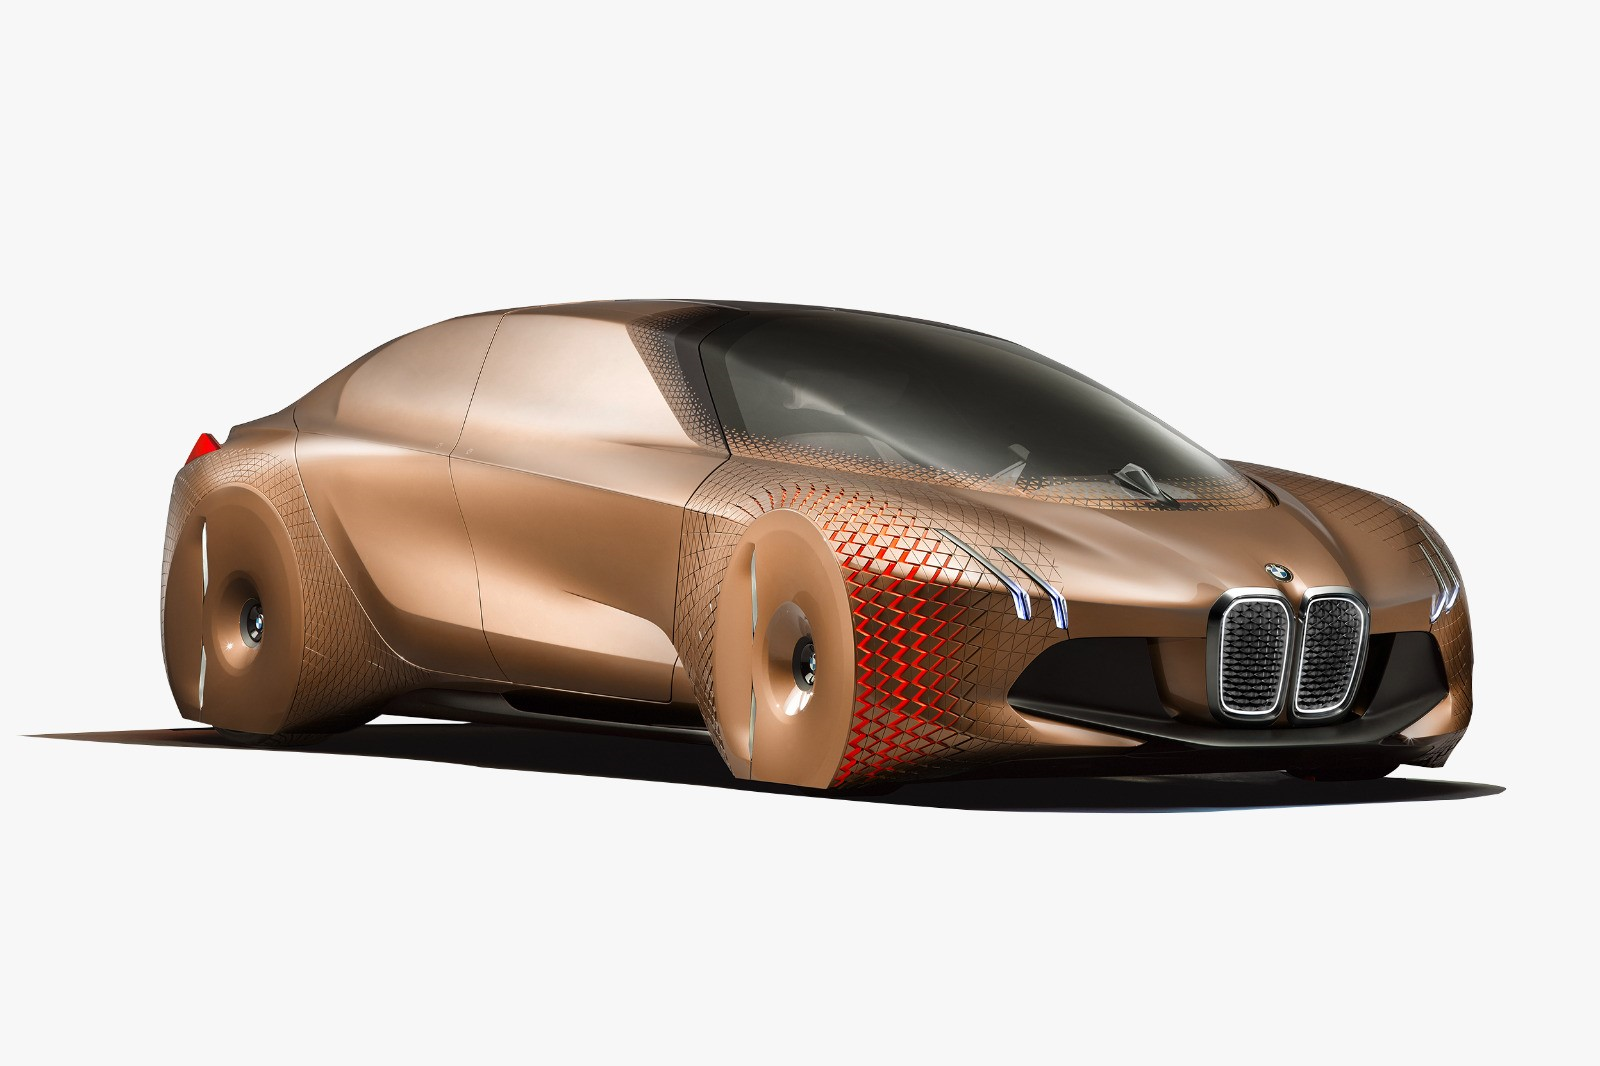
\includegraphics[scale=0.2]{images/bmw1.png}
			\end{center}
		\end{column}
		\begin{column}{0.6\textwidth}
		    \vspace{4mm}

			\textbf{Electric vehicles are the future}
			\begin{itemize}
				\item	Electric vehicles are increasing
				\item 	Tesla leading company
			\end{itemize}

			\vspace{8mm}

			\textbf{One big problem they all face}
			\begin{itemize}
				\item limited battery capacity
				\item a lot more recharges needed than regular\\``petrol'' vehicles
				\item vehicles need efficient charging managment\\and an EV Driver Interface
			\end{itemize}
		\end{column}
	\end{columns}

\end{frame}
\clearpage



\begin{frame}
\frametitle{Smart scheduling approach for EVs}

\begin{PraesentationAufzaehlung}
    \item \textbf{paper:} ``Smart Charging Schedules for Highway Travel with Electric Vehicles''
        \begin{itemize}
        \item authors: Victor del Razo and Hans-Arno Jacobsen
        \end{itemize}

    \item \textbf{idea:} EVs determine their charging stops during a highway trip

    \item \textbf{goal:} reduce the total travel time for each EV

    \item \textbf{summary:} shortest path problem
        \begin{itemize}
        \item A* search algorithm
        \item extended with verification of constraints
        \end{itemize}

    \item \textbf{software:} Python based simulation framework that provides
        \begin{itemize}
        \item generated trip data
        \item time-dependent parameters
        \end{itemize}

\end{PraesentationAufzaehlung}

\end{frame}
\clearpage



\begin{frame}
\frametitle{Smart scheduling approach for EVs}

\begin{PraesentationAufzaehlung}
    \item \textbf{simulation model}
        \begin{itemize}
        \item electric vehicles (EVs)
        \item charging stations (CSs)
        \item highway
        \end{itemize}

    \item \textbf{scheduling design}
        \begin{itemize}
        \item local to the EV
        \item communication with charging stations
        \item highway-related information system
        \end{itemize}

    \item \textbf{scheduling process}
        \begin{itemize}
        \item calculate set of charging stops and times
        \item submit bookings to the charging stations
        \item proceed trip as planned unless an update event is received
        \end{itemize}

\end{PraesentationAufzaehlung}

\end{frame}
\clearpage



\begin{frame}
\frametitle{Interactive Front-Ends}

Our task was to design and implement two front-ends for the simulation framework.

\begin{PraesentationAufzaehlung}

    \item \textbf{Simulation Manager Interface}
        \begin{itemize}
        \item show current states of EVs and CSs
        \end{itemize}

    \item \textbf{EV Driver Interface}
        \begin{itemize}
        \item show relevant vehicle information
        \item display travel-related information
        \end{itemize}

\end{PraesentationAufzaehlung}

\end{frame}
\clearpage



\begin{frame}
\frametitle{Research question}

What is the most suitable form of presentation for the data that is most relevant during the simulation and while
driving respectively?

\vspace{-8mm}
\begin{PraesentationAufzaehlung}

    \item \textbf{Simulation Manager Interface}
        \begin{itemize}
        \item data-heavy application
        \item structured data access
        \item relation between EVs and CSs
        \item schedule changes
        \item aggregated metrics
        \end{itemize}

    \item \textbf{EV Driver Interface}
        \begin{itemize}
        \item limited user attention
        \item separation of information
        \item time-relevant data
        \end{itemize}

\end{PraesentationAufzaehlung}
\vspace{-2mm}

Which tools, libraries, frameworks or APIs can be used to implement the two front-ends? \\
Which are most suitable for our purpose?

\end{frame}
\clearpage



\begin{frame}
	\frametitle{Requirements EV Driver Interface}

	\begin{PraesentationAufzaehlung}

		\item \textbf{Performance}
		\begin{itemize}
			\item real time data without delay
			\item if driver's attention is needed reduce distraction to a minimum
		\end{itemize}

		\item \textbf{Functional}
		\begin{itemize}
			\item functionality of the UI must be verified through measurment or testing
			\item UI missfunction etc. can lead to sevear damage e.g. missleading route
		\end{itemize}

		\item \textbf{Design}
		\begin{itemize}
			\item vehicles self status e.g. battery status at static position
			\item trip information like map components can be dynamic
			\item $\rightarrow$ simplistic desgin to avoid driver distraction and workload
		\end{itemize}

	\end{PraesentationAufzaehlung}
\end{frame}
\clearpage



\begin{frame}
	\frametitle{Requirements Simulation Manager Interface}

	\begin{PraesentationAufzaehlung}

		\item \textbf{Simulation Manager Interface}
		\begin{itemize}
			\item most important data first in sight e.g. charging stations, EV's
			\item detailed information hidden on first sight $\rightarrow$ reduce complexity
			\item real time data without much delay
		\end{itemize}

	\end{PraesentationAufzaehlung}

\end{frame}
\clearpage



\begin{frame}
	\frametitle{EV Driver Interface}

	Here JavaScript API

	\vspace*{-3mm}
	\begin{minipage}[t][0cm]{\paperwidth}%
		\hspace*{-\PraesentationSeitenrand}%
		\includegraphics[width=\paperwidth]{images/unser_interface.png}
	\end{minipage}

\end{frame}
\clearpage




\begin{frame}
	\frametitle{Here API vs Google Maps API comparison}

	Which API is most suitable for the EV Driver interface?

	\vspace{-8mm}
	\begin{PraesentationAufzaehlung}

		\item \textbf{Google Maps API}
		\begin{itemize}
			\item Turn-by-Turn Navigation is not possible
			\item Offline use is limited
		\end{itemize}

		\item \textbf{Here API}
		\begin{itemize}
			\item Developer friendly (full control of maps)
			\item Turn-by-Turn Navigation even offline
			\item $\rightarrow$ more suitable
		\end{itemize}

	\end{PraesentationAufzaehlung}
\end{frame}
\clearpage




\begin{frame}[fragile]
\frametitle{main.js}

\begin{minted}{javascript}
function calculateRouteFromAtoB(platform) {
    var router = platform.getRoutingService(),
    routeRequestParams = {
        mode: 'fastest;car',
        representation: 'display',
        routeattributes: 'waypoints,summary,shape,legs',
        maneuverattributes: 'direction,action',
        waypoint0: '48.2626,11.6679', // Brandenburg Gate
        waypoint1: '48.7752,11.4595', // Friedrichstrasse Railway Station
        waypoint2: '49.4268,11.1255' // Stadion Nuremberg
    };

    router.calculateRoute(
    routeRequestParams,
    onSuccess,
    onError
    );
}
\end{minted}

\end{frame}
\clearpage



\begin{frame}
\frametitle{Simulation Manager Interface}

Google Maps JavaScript API \\

\vspace*{-3mm}
\begin{minipage}[t][0cm]{\paperwidth}%
\hspace*{-\PraesentationSeitenrand}%
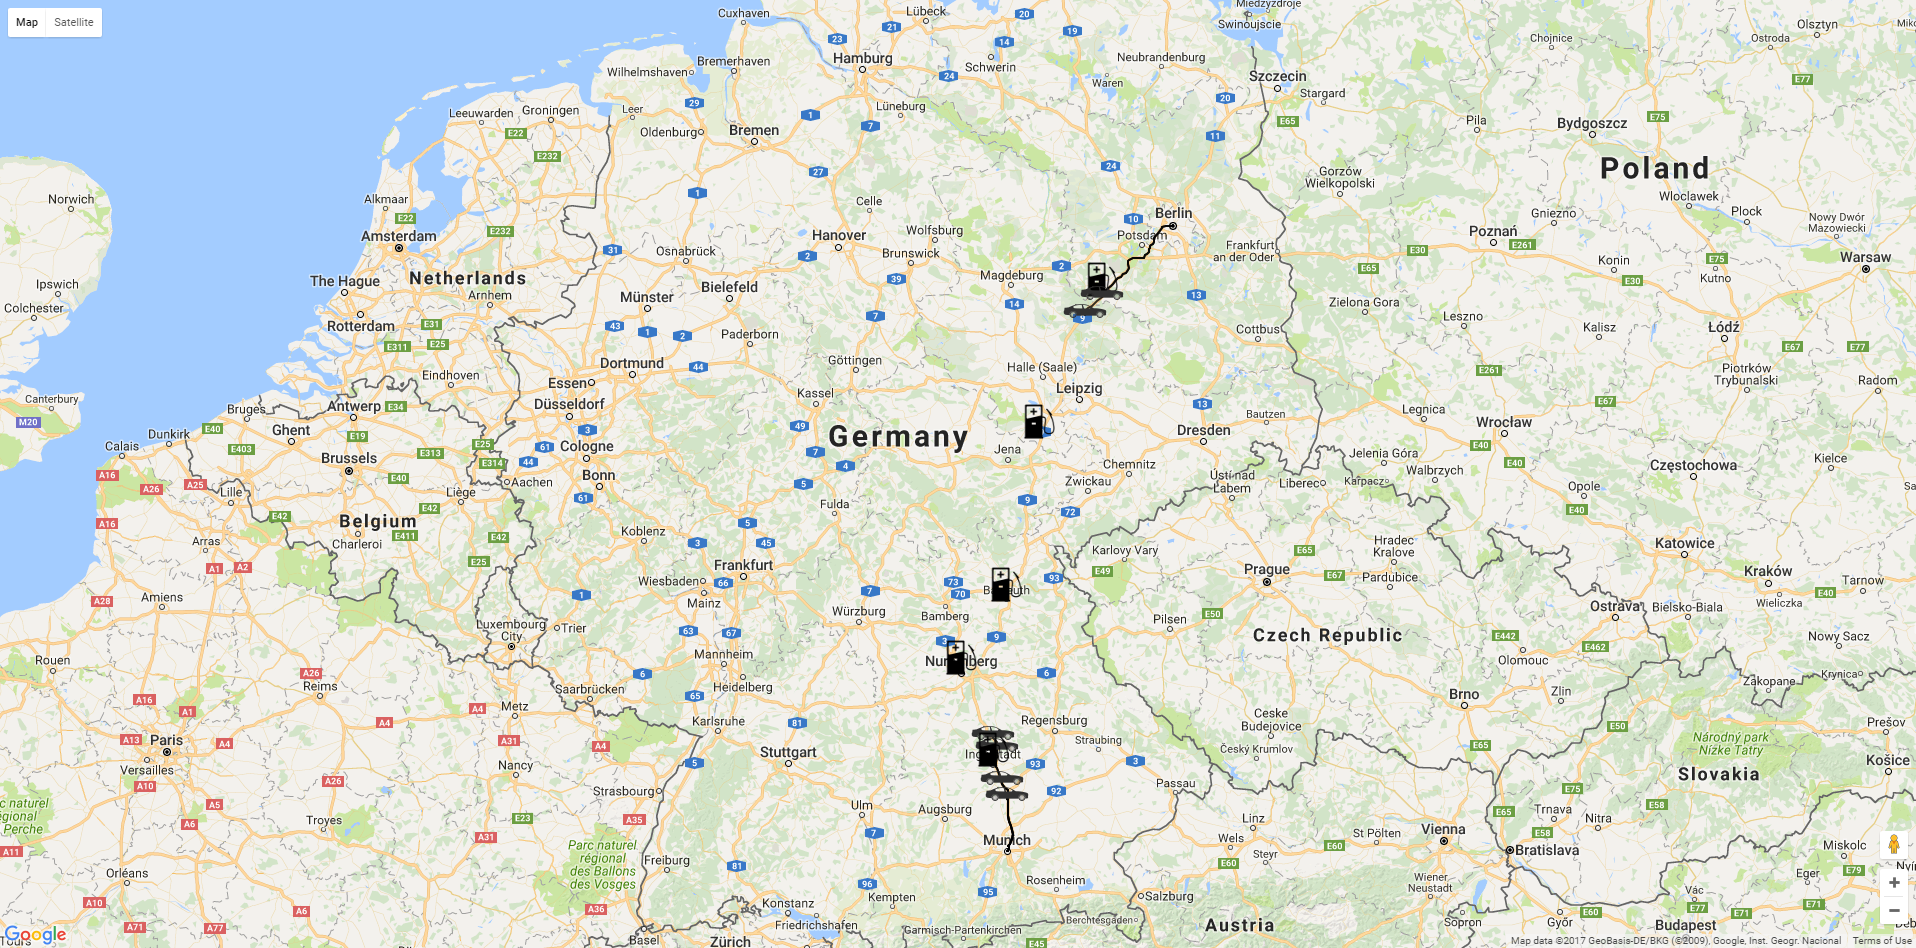
\includegraphics[width=\paperwidth]{images/simulation_manager.png}
\end{minipage}

\end{frame}
\clearpage



\begin{frame}[fragile]
\frametitle{config.js}

\begin{minted}{javascript}
var config = {
    mapID: "map",
    mapCenter: "Germany",
    mapZoom: 7,
    markers: {
        car: {
            url: "img/markers/car.png",
            anchor: new google.maps.Point(24, 18)
        },
        battery: {
            url: "img/markers/battery.png",
            anchor: new google.maps.Point(20, 36)
        }
    }
};
\end{minted}

\end{frame}
\clearpage



\begin{frame}[fragile]
\frametitle{main.js}

\begin{minted}{javascript}
$(document).ready(function () {

    // Init map
    var map = new Map();

    // Electric vehicles traveling from A to B
    var ev = [];

    ev.push(new EV(map.map, 1, 0, "Munich", "Berlin"));
    ev.push(new EV(map.map, 2, 10, "Munich", "Berlin"));
    ev.push(new EV(map.map, 3, 25, "Berlin", "Munich"));

    // Charging stations at location C
    var cs = [];

    cs.push(new CS(map.map, 1, "Ingolstadt"));
    cs.push(new CS(map.map, 2, "Nuremberg"));
    cs.push(new CS(map.map, 3, "Bayreuth"));
    cs.push(new CS(map.map, 4, "Osterfeld"));
});
\end{minted}

\end{frame}
\clearpage



\begin{frame}[fragile]
\frametitle{map.js}

\begin{minted}{javascript}
function Map() {
    this.init = function () {

        // Create new Google Map
        this.map = new google.maps.Map(document.getElementById(config.mapID), {
            mapTypeId: google.maps.MapTypeId.ROADMAP
        });

        // Center and fit country in viewport
        var geocoder = new google.maps.Geocoder();
        var map = this.map;

        geocoder.geocode({'address': config.mapCenter}, function (results, status) {
            if (status == google.maps.GeocoderStatus.OK) {
                map.setCenter(results[0].geometry.location);
                map.fitBounds(results[0].geometry.viewport);
            }
        });
    };
}
\end{minted}

\end{frame}
\clearpage



\begin{frame}[fragile]
\frametitle{cs.js – 1}

\begin{minted}{javascript}
function CS(map, id, location) {
    var CS = this;

    var stats = {
        id: id,
        time: '',
        queue_length: '',
        busy_poles_fc: '',
        busy_poles_tsc: '',
        arrived_cars: '',
        leaving_cars: '',
        queued_cars: '',
        plugged_cars: '',
        energy_consumed: '',
        energy_produced: '',
        energy_stored: '',
        energy_bought: '',
        queue_prediction_fc: '',
        queue_prediction_tsc: ''
    };
\end{minted}

\end{frame}
\clearpage



\begin{frame}[fragile]
\frametitle{cs.js – 2}

\begin{minted}{javascript}
    this.init = function () {
        var marker = new google.maps.Marker({
            map: map,
            icon: config.markers.battery
        });

        CS.setPosition(marker);

        var panel = new google.maps.InfoWindow({
            content: CS.getStats()
        });

        CS.initStats(panel, marker);
    };
\end{minted}

\end{frame}
\clearpage



\begin{frame}[fragile]
\frametitle{cs.js – 3}

\begin{minted}{javascript}
    this.getStats = function () {
        var info = '';

        for (var key in stats) {
            info += key + ': ' + stats[key] + '<br>';
        }

        return info;
    };
\end{minted}

\end{frame}
\clearpage



\begin{frame}[fragile]
\frametitle{ev.js – 1}

\begin{minted}{javascript}
function EV(map, id, start_time, origin, destination) {
    var EV = this;

    var stats = {
        id: id,
        time: '',
        position: '',
        geo_position: '',
        distance_travelled: '',
        time_travelled: '',
        time_waited: '',
        time_charged: '',
        time_driven: '',
        battery_level: '',
        speed: '',
        driving_flag: '',
        schedule_status: ''
    };
\end{minted}

\end{frame}
\clearpage



\begin{frame}[fragile]
\frametitle{ev.js – 2}

\begin{minted}{javascript}
    this.start = function () {
        var directions = new google.maps.DirectionsService();

        var request = {
            origin: origin,
            destination: destination,
            travelMode: google.maps.TravelMode.DRIVING
        };

        setTimeout(function () {
            directions.route(request, function (result, status) {
                if (status == google.maps.DirectionsStatus.OK) {
                    EV.autoUpdate(map, result.routes[0].legs);
                }
            });
        }, start_time * 1000);
    };
\end{minted}

\end{frame}
\clearpage



\begin{frame}[fragile]
\frametitle{ev.js – 3}

\begin{minted}{javascript}
    this.autoUpdate = function (map, legs) {
        var route, marker, panel;

        route = new google.maps.Polyline({
            path: [],
            geodesic: true,
            strokeColor: '#000000',
            strokeOpacity: 0.8,
            strokeWeight: 2,
            editable: false,
            map: map
        });

        marker = new google.maps.Marker({
            map: map,
            icon: config.markers.car
        });

        ...
\end{minted}

\end{frame}
\clearpage



\begin{frame}[fragile]
\frametitle{ev.js – 4}

\begin{minted}{javascript}
        ...

        var timeUnit = 0;

        for (var i = 0; i < legs.length; i++) {
            for (var j = 0; j < legs[i].steps.length; j++) {
                for (var k = 0; k < legs[i].steps[j].path.length; k++) {
                    setTimeout(function (coords) {

                        route.getPath().push(coords);
                        EV.moveMarker(map, marker, coords);
                        EV.updateStats(panel);

                    }, 50 * timeUnit++, legs[i].steps[j].path[k]);
                }
            }
        }
\end{minted}

\end{frame}
\clearpage
\usebackgroundtemplate{%
	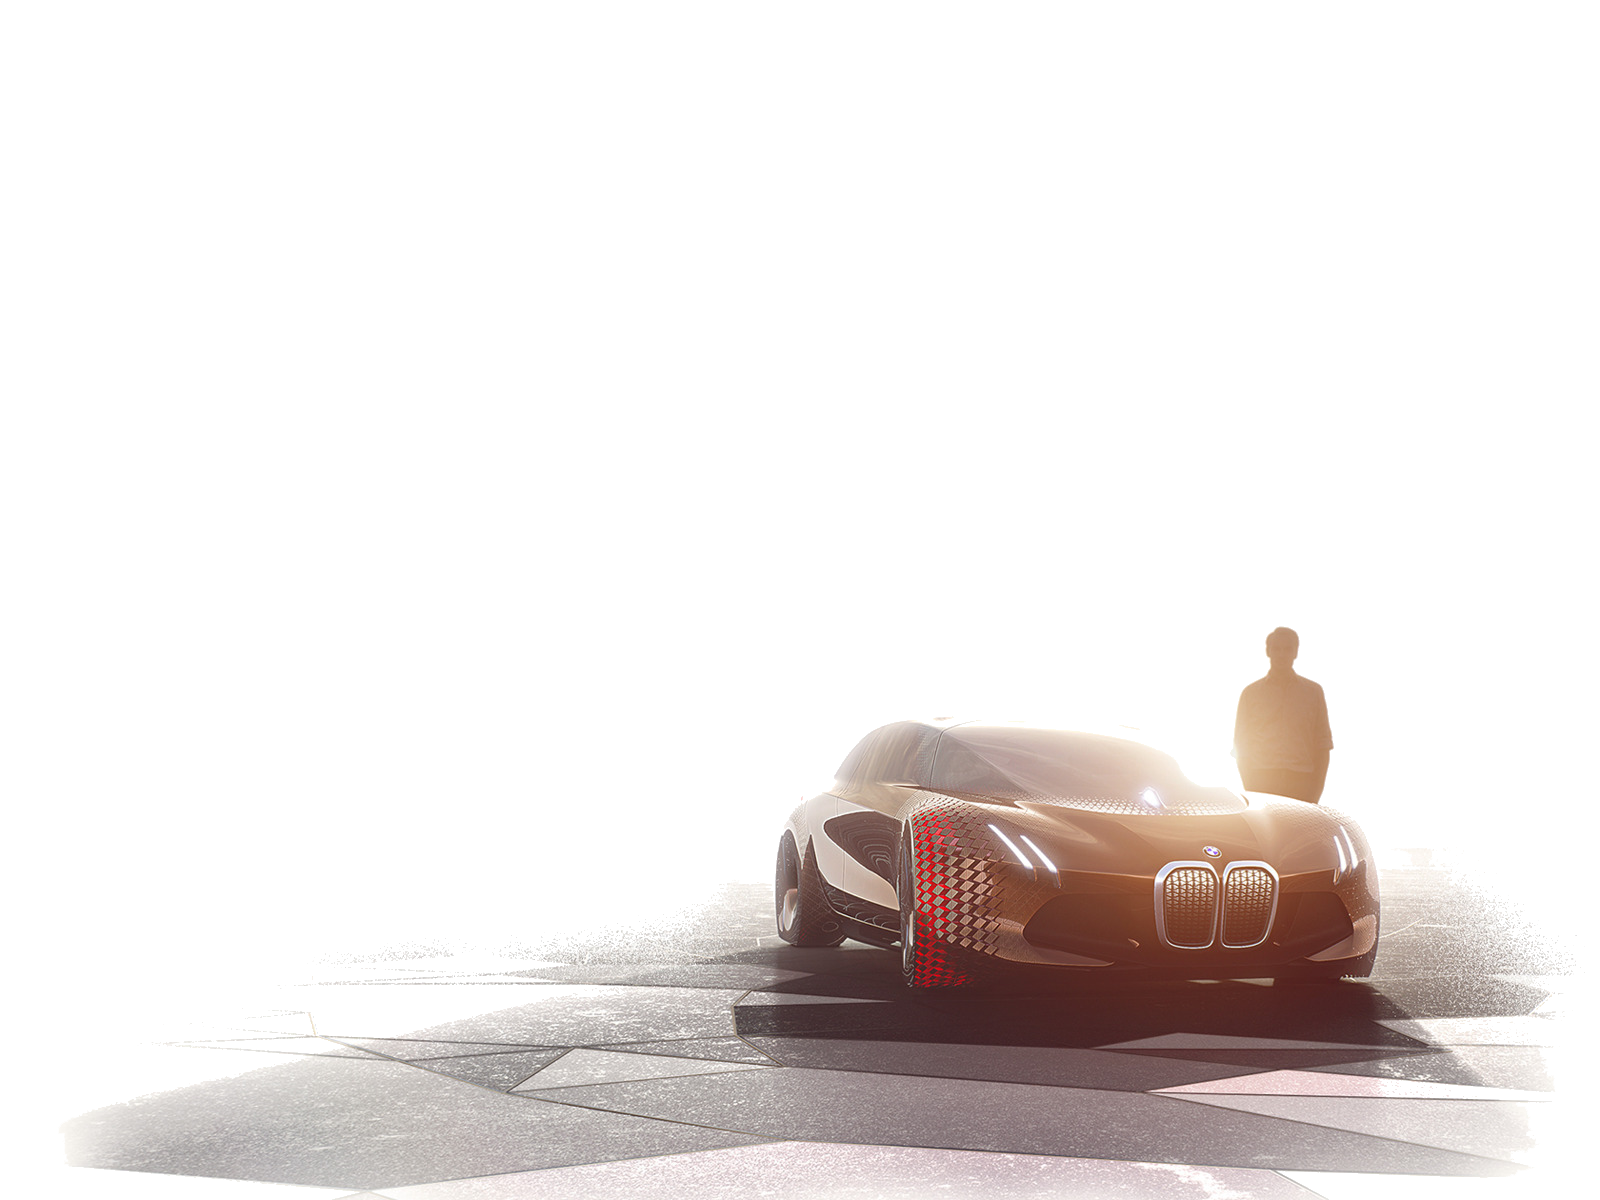
\includegraphics[width=\paperwidth,height=\paperheight]{images/bmw2.png}} 
\begin{frame}
	\frametitle{Outlook}
		\textbf{EV Driver Interface}
	\begin{itemize}
		\item	evtl. integration with the backend
		\item 	dynamic routing
	\end{itemize}
	
	\vspace{8mm}
	
	\textbf{Simulation managment}
	\begin{itemize}
		\item 
		\item 
		\item 
	\end{itemize}
	
\end{frame}
\clearpage